\documentclass[14pt, a4paper]{extarticle}

\usepackage{ProkhorovaGOST}
\usepackage{hyperref}
\usepackage{listings}
\usepackage{array}
\usepackage{caption}
\hypersetup{
	pdftex,
	colorlinks = true,
	linkcolor = black,
	filecolor = magenta,
	citecolor = green,      
	urlcolor = cyan,
}

% к таблице и листингу подпись сверху, перед каждым иллюстративным материалом анонсировать
% написатьт в квадратных скобках к рекурсии комментарием что это метод и понятно почему вызываем его снова
\definecolor{mylightgray}{RGB}{240,240,240}
\definecolor{mygreen}{rgb}{0,0.6,0}
\definecolor{mygray}{rgb}{0.5,0.5,0.5}
\definecolor{mymauve}{rgb}{0.58,0,0.82}

\lstset{
	backgroundcolor=\color{mylightgray},rulecolor=\color{red},  % choose the background color; you must add \usepackage{color} or \usepackage{xcolor}; should come as last argument
	basicstyle=\footnotesize\ttfamily,        % the size of the fonts that are used for the code
	breakatwhitespace=false,         % sets if automatic breaks should only happen at whitespace
	breaklines=true,                 % sets automatic line breaking
	captionpos=t,                    % sets the caption-position to bottom
	commentstyle=\color{mygreen},    % comment style
	extendedchars=false,              % lets you use non-ASCII characters; for 8-bits encodings only, does not work with UTF-8
	firstnumber=0,                % start line enumeration with line 1000
	frame=shadowbox,
	%rulesepcolor=\color{green},	                   % adds a frame around the code
	keepspaces=true,                 % keeps spaces in text, useful for keeping indentation of code (possibly needs columns=flexible)
	keywordstyle=\color{blue}\textbf,       % keyword style
	language=Python,                 % the language of the code
	morekeywords={*,...},            % if you want to add more keywords to the set
	numbers=left,                    % where to put the line-numbers; possible values are (none, left, right)
	numbersep=5pt,                   % how far the line-numbers are from the code
	numberstyle=\scriptsize\color{mygray}, % the style that is used for the line-numbers
	rulecolor=\color{black},         % if not set, the frame-color may be changed on line-breaks within not-black text (e.g. comments (green here))
	showspaces=false,                % show spaces everywhere adding particular underscores; it overrides 'showstringspaces'
	showstringspaces=false,          % underline spaces within strings only
	showtabs=false,                  % show tabs within strings adding particular underscores
	stepnumber=1,                    % the step between two line-numbers. If it's 1, each line will be numbered
	stringstyle=\color{mymauve},     % string literal style
	tabsize=4,	                   % sets default tabsize to 2 spaces
	title=\lstname                   % show the filename of files included with \lstinputlisting; also try caption instead of title
}
\usepackage{YATPR}

\usepackage{float}

\begin{document}
\begin{titlepage}
	\newgeometry{pdftex, left=2cm, right=2cm, top=2.5cm, bottom=2.5cm}
	\fontsize{12pt}{12pt}\selectfont
	\noindent \begin{minipage}{0.15\textwidth}
		
\includegraphics[width=\linewidth]{pictures/b_logo.jpg}
	\end{minipage}
	\noindent\begin{minipage}{0.9\textwidth}\centering
		\textbf{Министерство науки и высшего образования Российской Федерации}\\
		\textbf{Федеральное государственное бюджетное образовательное учреждение высшего образования}\\
		\textbf{«Московский государственный технический университет имени Н.Э.~Баумана}\\
		\textbf{(национальный исследовательский университет)»}\\
		\textbf{(МГТУ им. Н.Э.~Баумана)}
	\end{minipage}
	
	\noindent\rule{18cm}{3pt}
	\newline\newline
	\noindent ФАКУЛЬТЕТ $\underline{\text{«Информатика и системы управления»}}$ \newline\newline
	\noindent КАФЕДРА $\underline{\text{«Программное обеспечение ЭВМ и информационные технологии»}}$\newline\newline\newline\newline\newline\newline\newline
	
	
	\begin{center}
		\Large\textbf{Отчет по лабораторной работе №5}\newline
	\end{center}
	
	\noindent\textbf{Название} $\underline{\text{~Моделирование работы информационного центра~~~~~~~~~}}$\newline\newline\newline
	\noindent\textbf{Дисциплина} $\underline{\text{~Моделирование~~~~~~~~}}$\newline\newline
	\noindent\textbf{Студент} $\underline{\text{Зайцева А. А.~~~~~~~~~~~~~~~~~~~~~~~~~~~~~~~~~~~~~~~~~}}$\newline\newline
	\noindent\textbf{Группа} $\underline{\text{ИУ7-72Б~~~~~~~~~~~~~~~~~~~~~~~~~~~~~~~~~~~~~~~~~~~~}}$\newline\newline
	\noindent\textbf{Оценка (баллы)} $\underline{\text{~~~~~~~~~~~~~~~~~~~~~~~~~~~~~~~~~~~~~~~~~~~~~~~~~}}$\newline\newline
	\noindent\textbf{Преподаватель}$\underline{\text{~Рудаков И. В.~~~~~~~~~~}}$\newline
	
	\begin{center}
		\vfill
		Москва~---~\the\year
		~г.
	\end{center}
 \restoregeometry
\end{titlepage}


\setcounter{page}{2}
\section{Задание}
Изучить методы генерирования псевдослучайных чисел, а также критерии оценки случайности последовательности. Реализовать критерий оценки случайной последовательности. Сравнить результаты работы данного критерия на одноразрядных, двухразрядных и трехразрядных последовательностях целых чисел. Последовательности получать алгоритмическим и табличным способами. Предусмотреть возможность ввода десяти чисел для оценки их по критерию.

\section{Теоретическая часть}
Случайные числа — искусственно полученная последовательность реализаций случайной величины с заданным законом распределения.

На практике используется три основных способа получения случайных чисел:
\begin{itemize}
    \item Аппаратный
    \item Табличный(файловый)
    \item Алгоритмический(программный)
\end{itemize}

\textbf{Аппаратный способ получения случайных чисел}

Аппаратные генераторы случайных чисел – это устройства, использующие для создания случайных чисел замеры параметров некоторых физических процессов. Как правило, аппаратный генератор случайных чисел состоит из источника энтропии и устройства, преобразующего значения, полученные с источника энтропии, в нужный формат.

\textbf{Табличный способ получения случайных чисел}

В данном способе в качестве источника случайных чисел используют заранее подготовленные таблицы, содержащие проверенные некоррелированные числа. Недостатки такого способа: использование внешнего ресурса для хранения чисел, ограниченность последовательности, предопределенность значений.

\textbf{Алгоритмический способ получения случайных чисел}

Алгоритмический генератор является комбинацией физического генератора и детерминированного алгоритма. Такой генератор использует ограниченный набор данных, полученный с выхода физического генератора для создания длинной последовательности чисел преобразованиями исходных чисел. 
Из-за дороговизны аппаратных генераторов случайных чисел в большинстве случаев, в качестве источника энтропии используются ресурсы вычислительной машины, на которой выполняется программа генерации ПСЧ. При отсутствии аппаратного генератора случайных чисел в качестве источника энтропии могут использоваться:
\begin{itemize}
    \item состояние системных часов; 
    \item время задержек между нажатиями клавиш клавиатуры или движениями мышки; 
    \item содержимое буферов ввода/вывода; 
    \item значения, получаемые при работе системы.
\end{itemize}

\subsection{Выбранные методы}

Для получения случайных чисел алгоритмическим способом выбран линейный конгруэнтный метод.

\textbf{Линейный конгруэнтный метод}

Для осуществления генерации чисел данным методом, необходимо задать 4 числа:


m > 0,  модуль

%0 \leq a \leq m, множитель

%0 \leq c \leq m, приращение

%0 \leq $ X_{0}$ \leq m, начальное число


Последовательность случайных чисел генерируется при помощи формулы:

\begin{equation}
%X_{n + 1} = (a*X_{n} + c) \mod m, при n \geq 0
\end{equation}

При некоторых наборах чисел m, a, c, и $X_{0}$ последовательность не может быть "случайной". Поэтому важно правильно их подобрать. В конгруэнтной последовательности всегда существуют циклы - периоды, необходимо чтобы последовательность, которую мы используем, имела относительно длинный период.

Выбранный критерий оценки случайной последовательности - критерий "хи-квадрат". Это один из самых известных статистических критериев, также это основной метод, используемый в сочетании с другими критериями. 

С помощью этого критерия можно узнать, удовлетворяет ли генератор случайных чисел требованию равномерного распределения или нет. 
Для оценки по этому критерию необходимо вычислить статистику V по формуле:

\begin{equation}
    V = \frac{1}{n} \sum_{s = 1}^k (\frac{Y_{s}^2}{p_{s}}) - n
\end{equation}

где n – количество независимых испытаний, k – количество категорий, $Y_{s}$ — число наблюдений, которые действительно относятся к категории S, $p_{s}$ — вероятность того, что каждое наблюдение относится к категории s.  

Значение V является значением критерия «хи-квадрат» для экспериментальных данных. Приемлемое значение этого критерия можно определить по таблице 1. Для этого используем строку с v = k-1, где k = 10, 90, 900 для задания лабораторной.  P в этой таблице — это вероятность того, что экспериментальное значение Vэксп. будет меньше табулированного (теоретического) Vтеор. или равно ему. Ее также можно рассматривать как доверительную вероятность.

Если вычисленное V окажется меньше 1\% точки или больше 99\% точки, можно сделать вывод, что эти числа недостаточно случайные. Если V лежит между 1\% и 5\% точками или между 95\% и 99\% точками, то эти числа «подозрительны». Если V лежит между 5\% и 10\% точками или 90\%-95\% точками, то числа можно считать «почти подозрительными». Проверка по "хи-квадрат" критерию часто производится три раза и более с разными данными. Если по крайней мере два из трех результатов оказываются подозрительными, то числа рассматриваются как недостаточно случайные.

\begin{figure}[H]
\center{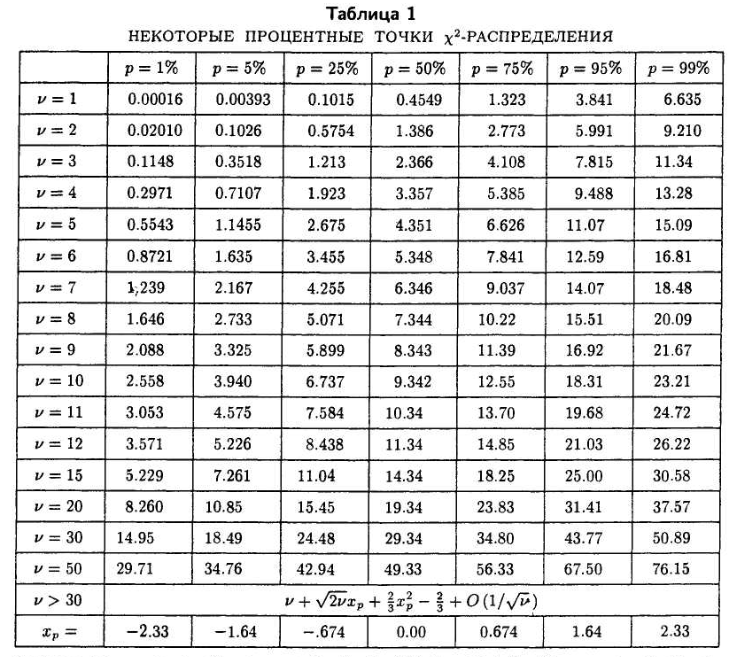
\includegraphics[scale=0.5]{pictures/table.png}}
\caption{Некоторые процентные точки "хи-квадрат" распределения (Источник: Кнут Д. Э. «Искусство программирования» ).}
\label{fig:table}
\end{figure}

\begin{table}[H]
\centering
\begin{tabular}{ | c | c | c | c | c | c | c | c |}
\hline
 k - 1 & p = 1\% & p = 5\% & p = 25\% & p = 50\% & p = 75\% & p = 95\% & p = 99\% \\ \hline
9 & 2.088 & 3.325 & 5.899 & 8.343 & 11.39 & 16.92 & 21.67 \\ \hline
89 & 60.93 & 68.25 & 79.68 & 88.33 & 97.60 & 112.02 & 122.94 \\ \hline
899 & 803.31 & 830.41 & 870.05 & 898.33 & 927.23 & 969.86 & 1000.57 \\ \hline
\end{tabular}
\caption{Таблица значений Vтеор для количества степеней свободы по заданию}
\end{table}

\section{Результаты работы программы}

Программа, реализованная в лабораторной работе, выводит на экран таблицу из 7 столбцов и 13 строк. 10 строк представлены для того, чтобы можно было пронаблюдать, какие числа возвращает генератор случайных чисел. Для каждого из реализованных методов в таблице есть по три столбца для чисел с разным количеством разрядов. В строке "коэффициент" выводится значение V, подсчитанное для каждого столбца (N = 10000). В последней строке выводится заключение, сделанное в результате анализа вычисленного значения по таблице 1.

Так же есть возможность ввести собственную последовательность и проанализировать ее. 

На рисунках \ref{fig:pic1}, \ref{fig:pic2}, \ref{fig:pic3} приведен пример трех запусков программ.

\begin{figure}[H]
\center{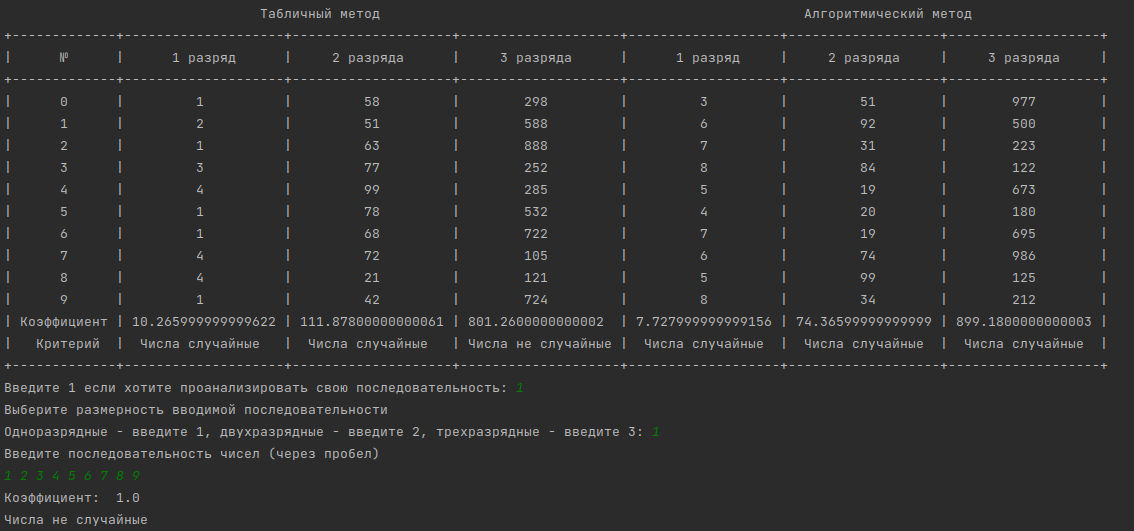
\includegraphics[scale=0.4]{pictures/pic1.png}}
\caption{Результат работы первого запуска программы}
\label{fig:pic1}
\end{figure}

\begin{figure}[H]
\center{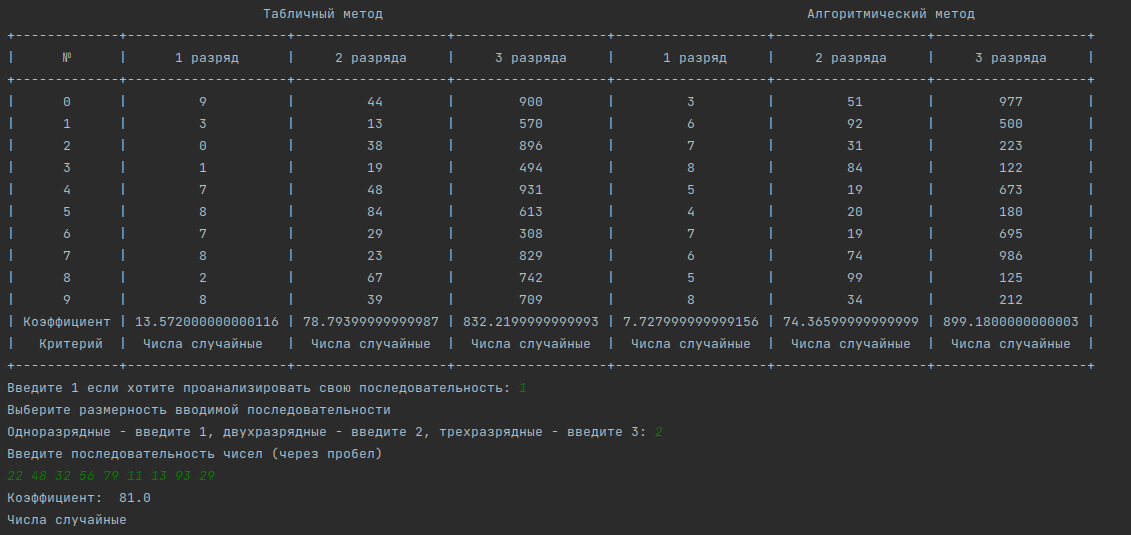
\includegraphics[scale=0.4]{pictures/pic2.png}}
\caption{Результат работы второго запуска программы}
\label{fig:pic2}
\end{figure}

\begin{figure}[H]
\center{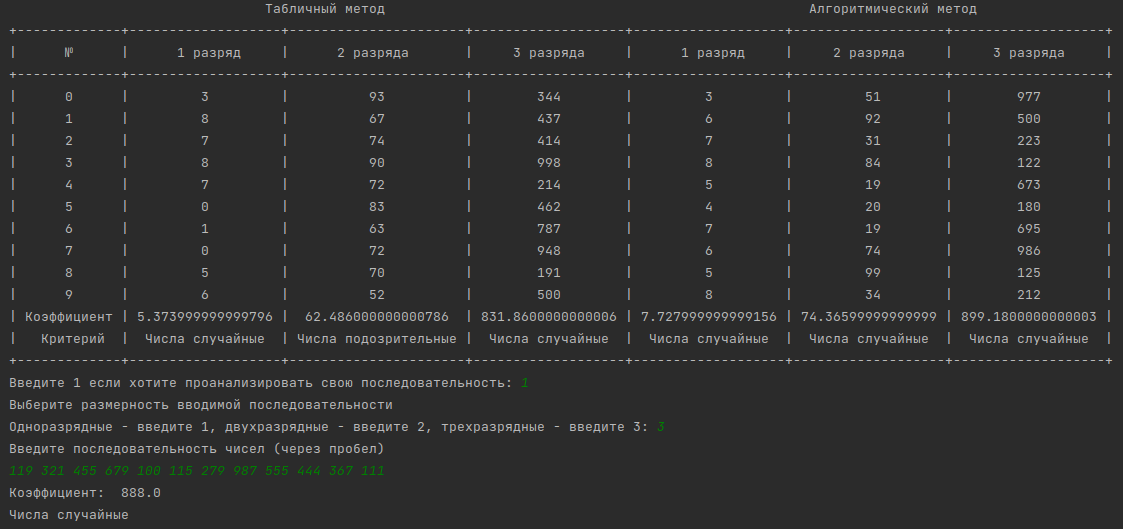
\includegraphics[scale=0.4]{pictures/pic3.png}}
\caption{Результат работы третьего запуска программы}
\label{fig:pic3}
\end{figure}

Проанализируем три выведеных результата для каждого столбца для того чтобы сделать вывод об эффективности генератора случайных чисел.

\textbf{Табличный способ получения случайных чисел}
\begin{itemize}
    \item Одноразрядные числа - во всех трех экспериментах числа в последовательности случайные, соответсвенно одноразрядные числа, генерируемые с помощью табличного метода являются случайными при оценке критерием "хи-квадрат".
    \item Двухразрядные числа - в двух экспериментах числа в последовательности случайные, в одном подозрительные. Так как количество экспериментов с ответом что числа подозрительные не 2 и не 3, то можно считать, что двухразрядные числа, генерируемые с помощью табличного метода являются случайными при оценке критерием "хи-квадрат".
    \item Трехразрядные числа - в двух экспериментах числа в последовательности случайные, в одном не являются случайными. Так как количество экспериментов с ответом что числа не случайные только 1 из 3, то можно считать это некоторой случайностью при генерации, которая не является закономерной. (После данного эксперимента было проведено еще 20 экспериментов которые не отражены в отчете и каждый раз получался ответ - числа случайные). Можно считать что трехразрядные числа, генерируемые с помощью табличного метода являются случайными при оценке критерием "хи-квадрат".
\end{itemize}

\textbf{Алгоритмический способ получения случайных чисел}

Во всех трех экспериментах и для одноразрядных, и для двухразрядных, и для трехразрядных чисел было установлено, что они случайные. 

Помимо таблиц на рисунках \ref{fig:pic1}, \ref{fig:pic2}, \ref{fig:pic3} представлен пример обработки последовательности, введенной пользователем. 

Так как иногда числа, сгенерированные с помощью табличного способа получения случайных чисел оказывались не случайными или подозрительными, то можно считать что алгоритмический способ получения случайных чисел эффективнее.

\section{Код программы}

Программа разработана в интегрированной среде разработки для языка программирования Python - PyCharm. 
В листинге 1 приведена реализация лабораторной работы.

\begin{lstlisting}[label=lst:list1]
from prettytable import PrettyTable
from itertools import islice

COUNT = 10000
m = 2. ** 31
a = 1664525
c = 1013904223

theor_koef_one_digit = {'1': 2.088, '5': 3.325, '25': 5.899, '50': 8.343, '75': 11.39, '95': 16.92, '99': 21.67}
theor_koef_two_digits = {'1': 60.93, '5': 68.25, '25': 79.68, '50': 88.33, '75': 97.60, '95': 112.02, '99': 122.94}
theor_koef_three_digits = {'1': 803.31, '5': 830.41, '25': 870.05, '50': 898.33, '75': 927.23, '95': 969.86, '99': 1000.57}
theor_koefs = {'one_digit': theor_koef_one_digit, 'two_digits': theor_koef_two_digits, 'three_digits': theor_koef_three_digits}

class RandomGenerator:
    def __init__(self):
        self.current = 10

    def get_random_number(self, low, high):
        self.current = (a * self.current + c) % m
        result = int(low + self.current % (high - low))
        return result

def table_rand():
    numbers = set()
    with open('digits.txt') as file:
        line_num = 0
        lines = islice(file, line_num, None)
        for l in lines:
            numbers.update(set(l.split(" ")[1:-1]))
            line_num += 1
            if len(numbers) >= 3 * COUNT + 1:
                break
        numbers.remove("")
        numbers = list(numbers)[:3 * COUNT]
    one_digit = [int(i) % 10 for i in numbers[:COUNT]]
    two_digits = [int(i) % 90 + 10 for i in numbers[COUNT:COUNT * 2]]
    three_digits = [int(i) % 900 + 100 for i in numbers[COUNT * 2:3 * COUNT]]
    return one_digit, two_digits, three_digits


def alg_rand():
    random = RandomGenerator()
    one_digit = [random.get_random_number(0, 10) for i in range(COUNT)]
    two_digits = [random.get_random_number(10, 100) for i in range(COUNT)]
    three_digits = [random.get_random_number(100, 1000) for i in range(COUNT)]
    return one_digit, two_digits, three_digits


def calc_hi(arr, start, end):
    n = len(arr)
    tab = [0 for i in range(start + end)]
    for i in range(n):
        tab[arr[i]] += 1
    s = 0
    for i in tab:
        s += i * i
    return s * (end - start) / n - n

def check_with_criterion(prac_koef, digit_str):
    if prac_koef < theor_koefs[digit_str]['1'] or prac_koef > theor_koefs[digit_str]['99']:
        return "Числа не случайные"

    if prac_koef >= theor_koefs[digit_str]['1'] and prac_koef <= theor_koefs[digit_str]['5']:
        return "Числа подозрительные"

    if prac_koef <= theor_koefs[digit_str]['99'] and prac_koef >= theor_koefs[digit_str]['95']:
        return "Числа подозрительные"
    return "Числа случайные"
def main():
    numbers = [i for i in range(10)]
    table_tbl = PrettyTable()
    one_tbl, two_tbl, three_tbl = table_rand()

    table_tbl.add_column("№", numbers)
    table_tbl.add_column('1 разряд', one_tbl[:10])
    table_tbl.add_column('2 разряда', two_tbl[:10])
    table_tbl.add_column('3 разряда', three_tbl[:10])

    one_alg, two_alg, three_alg = alg_rand()
    table_tbl.add_column('1 разряд', one_alg[:10])
    table_tbl.add_column('2 разряда', two_alg[:10])
    table_tbl.add_column('3 разряда', three_alg[:10])

    koef_tbl_one = calc_hi(one_tbl, 0, 10)
    koef_tbl_two = calc_hi(two_tbl, 10, 100)
    koef_tbl_three = calc_hi(three_tbl, 100, 1000)
    koef_alg_one = calc_hi(one_alg, 0, 10)
    koef_alg_two = calc_hi(two_alg, 10, 100)
    koef_alg_three = calc_hi(three_alg, 100, 1000)

    table_tbl.add_row(['Коэффициент', koef_tbl_one, koef_tbl_two, koef_tbl_three, koef_alg_one, koef_alg_two, koef_alg_three])

    table_tbl.add_row(['Критерий',
                      check_with_criterion(koef_tbl_one, 'one_digit'),
                      check_with_criterion(koef_tbl_two, 'two_digits'),
                      check_with_criterion(koef_tbl_three, 'three_digits'),
                      check_with_criterion(koef_alg_one, 'one_digit'),
                      check_with_criterion(koef_alg_two, 'two_digits'),
                      check_with_criterion(koef_alg_three, 'three_digits')])
    print("\t\t\t                    Табличный метод\t\t\t\t\t                                    Алгоритмический метод")

    print(table_tbl)

    flag = input("Введите 1 если хотите проанализировать свою последовательность: ")
    if flag == '1':
        print("Выберите размерность вводимой последовательности")
        digit_str = input("Одноразрядные - введите 1, двухразрядные - введите 2, трехразрядные - введите 3: ")
        arr = []
        if digit_str in ['1', '2', '3']:
            print("Введите последовательность чисел (через пробел)")
            arr_str = list(input().split())
            for digit in arr_str:
                if len(digit) != int(digit_str):
                    print("Некорректная разрядность")
                    return
                try:
                    d = int(digit)
                except:
                    print("Некорректное значение")
                    return
                arr.append(d)
            if digit_str == '1':
                hi_koef = calc_hi(arr, 0, 10)
            elif digit_str == '2':
                hi_koef = calc_hi(arr, 10, 100)
            else:
                hi_koef = calc_hi(arr, 100, 1000)
            print("Коэффициент: ", hi_koef)
            s = ['one_digit', 'two_digits', 'three_digits']
            print(check_with_criterion(hi_koef, s[int(digit_str) - 1]))
        else:
            print("Некорректный ввод")
            return

if __name__ == '__main__':
    main()

\end{lstlisting}
\end{document}